%% This is an example first chapter.  You should put chapter/appendix that you
%% write into a separate file, and add a line \include{yourfilename} to
%% main.tex, where `yourfilename.tex' is the name of the chapter/appendix file.
%% You can process specific files by typing their names in at the 
%% \files=
%% prompt when you run the file main.tex through LaTeX.
\chapter{Rincian Anggaran Penelitian}
% Rincian anggaran penelitian mencakup jumlah dana penelitian yang dibutuhkan beserta penggunaanya
% secara wajar, namun tidak termasuk hal-hal sebagai berikut:
%  Dana untuk pembelian aset, seperti alat-alat laboratorium, komputer, dll
%  Dana honorarium
%  Dana untuk biaya perjalanan dan akomodasi (selain untuk pengambilan sampel)

% Jumlah Anggaran Total: Rp 99.500.000 \\
% Bahan habis pakai: Rp 39.500.000\\ % internet, electric power, hosting web-server, stationery
% Sewa laboratorium/alat: Rp 60.000.000 \\ % lab, computer
% Lainnya, sebutkan: Rp 0 \\

Rincian anggaran belanja untuk penelitian disajikan dalam tabel dalam gambar~\ref{fig:rab}.

\begin{figure}
	\centering
	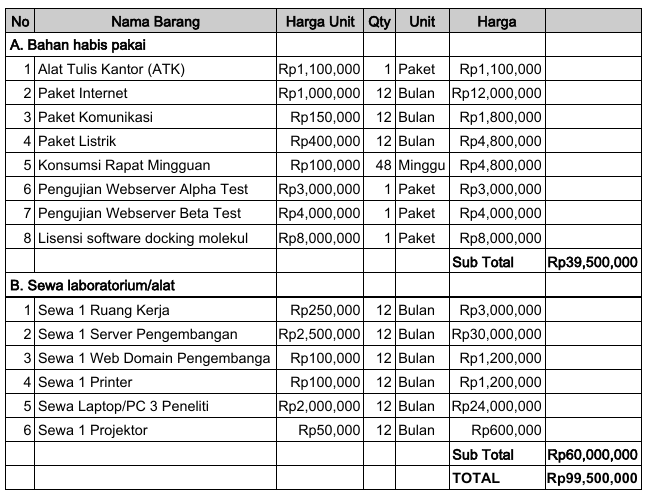
\includegraphics[scale=0.85, angle=0]{pics/rab.png}
	% 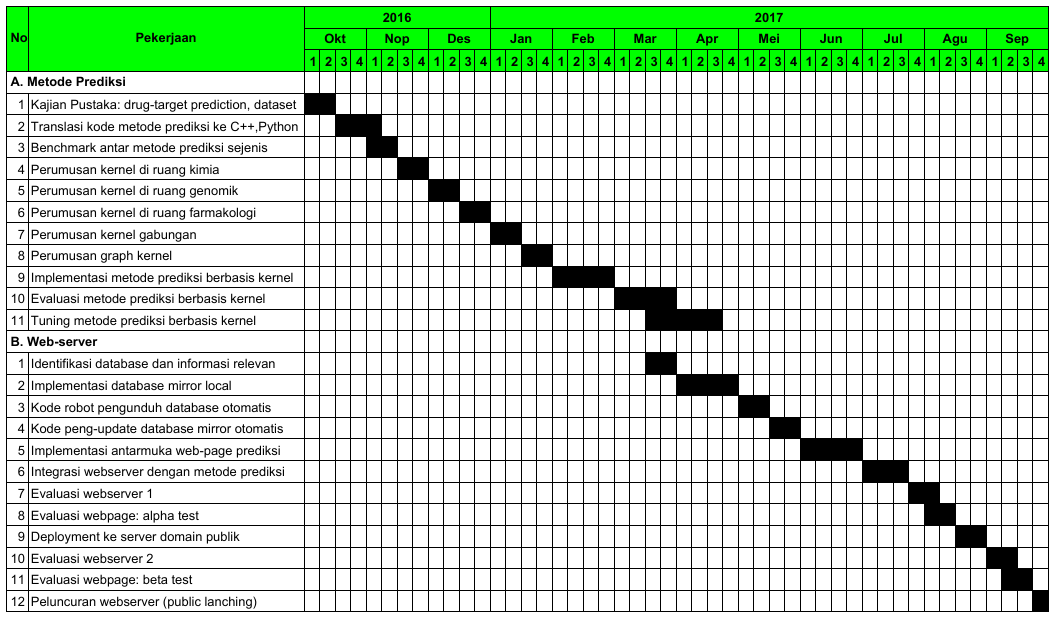
\includegraphics[width=\columnwidth]{pics/timeline.png}
 	\caption{Rincian anggaran belanja untuk penelitian.}
  	\label{fig:rab}
\end{figure}  